\chapter{Resumen completo}
Un árbol filogenético tiene las especies de interés en los nodos terminales y sus relaciones mostradas por las ramas. Los nodos internos representan hipotéticos taxones extintos. Hay un grupo externo que sirve para enraizar el árbol.

\begin{figure}[htbp]
\centering
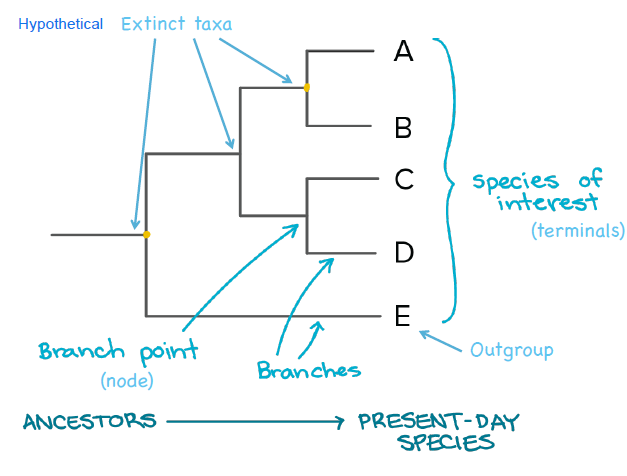
\includegraphics[width=0.7\linewidth]{figs/parts-phylotree.png}
\end{figure}

Hay distintos tipos de árbol:
\begin{itemize}
\item \textbf{Cladograma:} es una representación simple que es aceptable en matrices morfológicas. No muestra hipótesis evolutivas al no contener información sobre la relación entre ancestros y descendientes o cuánto han cambiado los descendientes a lo largo del tiempo.
\item \textbf{Filograma:} es un árbol en el que la longitud de las ramas indica la cantidad de cambios evolutivos inferidos del análisis.
\item \textbf{Cronograma:} se utiliza el tiempo para calcular las variaciones en los nodos mediante el empleo de relojes moleculares.
\end{itemize}

\begin{figure}[htbp]
\centering
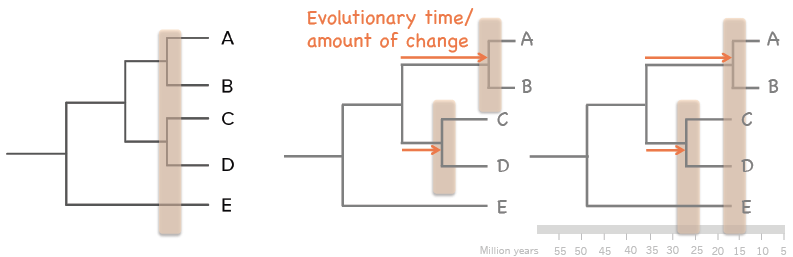
\includegraphics[width=0.7\linewidth]{figs/tree-types.png}
\end{figure}

Los árboles filogenéticos pueden tener ramas rotadas sin que cambie el mensaje. También hay distintas representaciones de los árboles que significan lo mismo. La diferencia está cuando un árbol está o no enraizado.

Se distinguen tres grupos de taxones en un árbol filogenético:
\begin{itemize}
\item \textbf{Monofilia:} todos los taxones que se originan de un mismo ancestro.
\item \textbf{Parafilia:} un ancestro, pero no todos sus descendientes.
\item \textbf{Polifilia:} algunos taxones de distintos ancestros.
\end{itemize}

\begin{figure}[htbp]
\centering
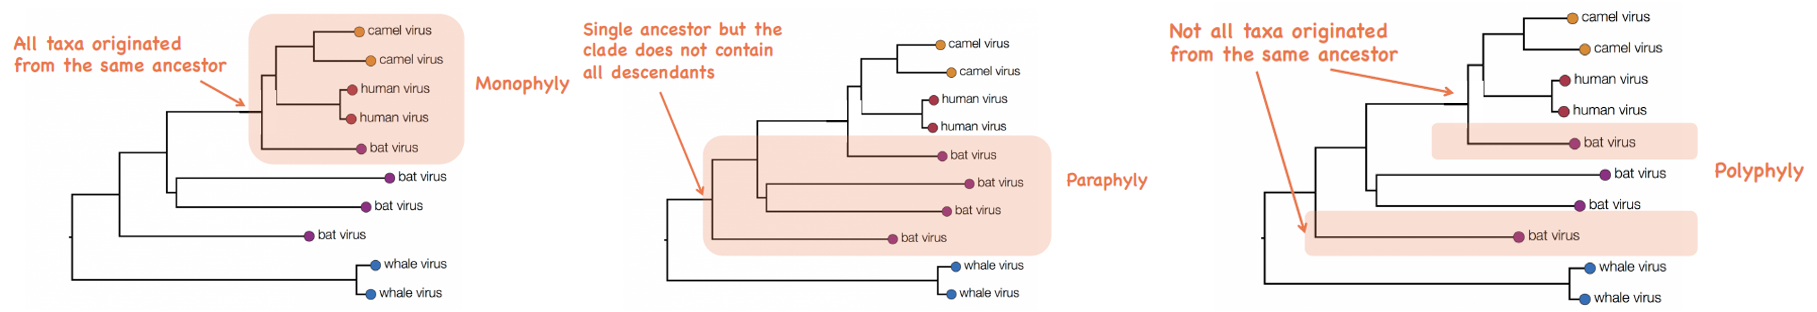
\includegraphics[width=\linewidth]{figs/tree-groups.png}
\end{figure}

Para construir un árbol filogenético, se necesitan elegir los taxones. Esto es decisión nuestra, pero hay que intentar no tener sesgos y elegir un buen ingroup y outgroup. Los tipos de datos también los podemos elegir en función de lo que está disponible. En cuanto a la cantidad de marcadores, depende del presupuesto que haya, pero se debe intentar tener los máximos posibles por PCR u otros. Se debe elegir un programa de alineamiento (MAFFT, Muscle, etc) y un modelo de evolución (jModelTest). No todos los genes evolucionan o mutan al mismo tiempo y de la misma forma, ya que depende de parámetros como el contenido GC, el tamaño genómico, el tiempo de generación, los niveles de expresión, los genes codificantes, la posición en el genoma, entre muchos otros. Por tanto, cada gen va a tener su propio modelo de sustitución, que difiere en los parámetros que describen las tasas de sustitución de cada nucleótido durante la evolución. Todas las mutaciones son posibles, pero con diferentes frecuencias dependiendo de si se trata de una transición o una transversión. Finalmente se debe elegir un método filogenético (por ejemplo, máxima verosimilitud + inferencia bayesiana) y la medición de confianza (bootstrap, convergencia, etc). 

Entre los métodos filogenéticos hay:
\begin{itemize}
\item \textbf{Máxima parsimonia:} asume que el árbol verdadero contiene el menor número de mutaciones posible, es decir, tiene la solución más parsimoniosa. Dado un set de secuencias (evidencia parcial), es necesario encontrar las secuencias ancestrales para construir un árbol enraizado y estimar el mínimo número de cambios contenidos en las ramas. No obstante, esto supone un problema computacional al no conocerse algoritmo, por lo que todos los modelos utilizan versiones simplificadas. Por ejemplo, la parsimonia ponderada emplea una puntuación diferente para cada cambio (transición/transversión) y puntuación diferente para cada posición. Para calcular la máxima parsimonia de forma manual, se emplea el algoritmo de Fitch para encontrar el estado ancestral: primero se va de descendientes al ancestro y luego del ancestro a los descendientes.
\item \textbf{Máxima verosimilitud:} la verosimilitud se define como la probabilidad de producir los datos observados por un modelo dados los parámetros. Es uno de los métodos más poderosos al poder utilizar modelos de sustitución (modelos evolutivos), corrige múltiples sustituciones y permite estimar la longitud de la rama, que indica la cantidad de cambios desde el ancestro. El problema de la máxima verosimilitud es la atracción de las ramas largas, un fenómeno que se produce cuando se infiere que los linajes que evolucionan rápidamente están estrechamente relacionados, independientemente de sus verdaderas relaciones evolutivas.
\item \textbf{Inferencia bayesiana:} basado en el teorema de Bayes, el enfoque bayesiano combina la probabilidad a priori de un árbol P(A) con la probabilidad de los datos (B) para producir una distribución de probabilidad posterior de los árboles P(A|B). La verosimilitud da la probabilidad de los datos dada la hipótesis y la bayesiana le da la probabilidad de la hipótesis dados los datos. Por ello, se habla de probabilidad posterior, y utiliza el algoritmo MCMC. Este algoritmo empieza en algún sitio, el cual tiene una verosimilitud y una probabilidad previa. Aleatoriamente se propone un nuevo estado (ajustando la longitud de una rama), y si la verosimilitud * probabilidad previa mejora, la cadena va allí. Después se calcula la relación de la probabilidad posterior entre el estado actual y el estado previo, que es entre 0 y 1. Se elije un número aleatorio entre esos valores y, si ese número tiene una probabilidad mejor que la relación de estados, se acepta el cambio. Así es como la cadena atraviesa los valles de probabilidad.
\end{itemize}

\begin{figure}[htbp]
\centering
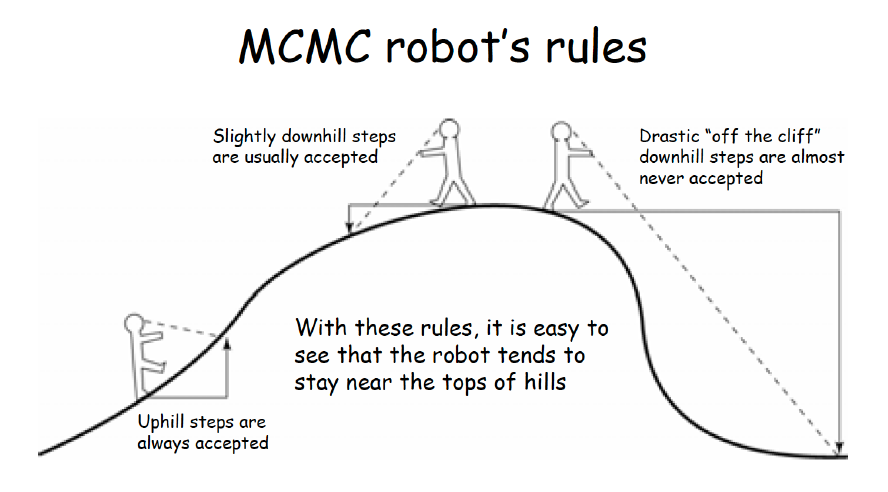
\includegraphics[width=0.6\linewidth]{figs/mcmc-rules.png}
\end{figure}

También hay varias maneras de evaluar la confianza:
\begin{itemize}
\item \textbf{Soporte de Bremer [> 70\%]:} diferencia en las longitudes de las ramas cuando se eliminan los clados (solo en parsimonia).
\item \textbf{Jackknife [> 70\%]:} probabilidad de que un clado se observe en todos los árboles (parsimonia).
\item \textbf{Bootstrap [> 70\%]:} probabilidad de que un clado se observe en todos los árboles (máxima verosimilitud).
\item \textbf{Probabilidad posterior [> 0.95]:} probabilidad de que un clado sea asignado bajo las condiciones muestradas (inferencia bayesiana).
\item \textbf{Convergencia:} evaluar si todas las cadenas (MCMC) convergen en la misma
solución (inferencia bayesiana).
\end{itemize}